\chapter[Processes]{Processes \\ \Large \textnormal{Group Milestone}}

\section{Introduction}

In computer science, a \href{https://en.wikipedia.org/wiki/Process_(computing)}{\texttt{process}} refers to an instance of a computer program that is being executed. It represents the \texttt{running state} of a program along with its associated \texttt{resources}, such as memory, files, and input/output devices. A process is an \texttt{isolated entity} with its own address space, allowing it to operate independently of other processes. It is managed by the operating system, which schedules and allocates resources to processes, ensuring their proper execution and coordination within the system. In other words, process are a \texttt{virtualization mechanism} for the cpu.

Our operating system can only run a simple process for the moment. It is time to extend it so that it is able to run several processes in parallel. The first part explains the creation of a process and the subtleties. The second part talks about \texttt{process management}. Once an operating system has several processes, there are two questions that become central. The first one is how to divide the computing power (cycles in the processors) between the different processes that are executed. The second is how to manage the whole process life cycle. Launching it is certainly an important step, but it must be possible to stop it and eventually resume it later. Once finished, you also have to clean up the resources. Below is an illustration of the complexity of this problem and the UNIX solution. 

\subsection{Technical words and concepts used in this section}

\subsubsection{Dispatcher}

The \texttt{Barrelfish CPU driver} utilizes a \texttt{capability} type known as a \texttt{dispatcher control block (DCB)} to encapsulate all relevant information about a process assigned to a specific core (dispatcher). When a process is spawned, it creates a\texttt{DCB} and subsequently provides it to the \texttt{CPU driver}. This designated memory area serves as a storage for various details pertaining to the process. For instance, it holds information such as the register state during a \texttt{context switch} and the error handlers to be invoked in the event of page faults.

\subsubsection{Elf image}

An \texttt{ELF (Executable and Linkable Format)} image refers to a common file format used for \texttt{executable files}, \texttt{object code} and \texttt{shared libraries} in many Unix-like operating systems. It serves as a \texttt{standardized} format for representing binary files that can be executed directly by a computer's processor or linked with other modules during the compilation and building process.

ELF images typically contain the compiled machine code, data, and other necessary information for an executable program or shared library. They consist of several sections, such as the program header table, which provides details about the layout and memory requirements of the executable, and the section header table, which defines individual sections containing different types of data (e.g., code, data, symbols, etc.).

\section{Starting a new process}

The process of initiating a a new process involves a series of sequential steps that need to be carried out. Initially, we embark upon the task of loading our elf binary into the memory. Following that, we proceed with establishing the \texttt{capability space}, ensuring that it is properly configured and ready for use. In the subsequent phase, we set up the \texttt{virtual address space}, ensuring that the necessary mappings and translations are in place inside of the page tables entries. Moving forward, we engage in the process of \texttt{parsing} our \texttt{binary image}, meticulously extracting the relevant information and structuring it appropriately. This part was very tricky and with a lot of subtleties. Subsequently, we set up the dispatcher and configure it by filling various fiend inside of the structure. Only once each of these steps has been successfully executed, are we able to \texttt{invoke} the dispatcher, initiating in the operation system the newly created process.

\subsection{Setup the capability space}

A process cannot generate something out of nothing; that would be considered magical. It requires a specific amount of RAM and certain abilities to effectively handle its virtual address space. To achieve this, we generate multiple capabilities, each with its own designated function.

The procedure for creating a capability is as follows: Initially, we must generate a capability within the parent process (for instance, a RAM-type capability). Next, we assign an address within the child's capability space. The final step involves \texttt{transferring} the capability from the parent to the child. The provided example illustrates how this is accomplished in the context of Barrelfish.


\begin{lstlisting}[caption={Typical process of creation and mapping of capability},language=C,frame=single,breaklines]
struct capref physical_chunk;
size_t        frame_size = 1024 * 1024;

err = ram_alloc(&physical_chunk, frame_size);
if (err_is_fail(err)) {
    return err_push(err, LIB_ERR_FRAME_ALLOC);
}

struct capref earlymem_capref = {
    .cnode = *rootcn_slot_taskcn,
    .slot  = TASKCN_SLOT_EARLYMEM,
};

err = cap_copy(earlymem_capref, physical_chunk);
if (err_is_fail(err)) {
    return err_push(err, LIB_ERR_CAP_COPY);
}
\end{lstlisting}

We have several capabilities that require mapping. Firstly, we need a self-capability for inter-core communication purposes. Additionally, we require a capability for the dispatcher, another one for the root L1 node, and one for the dispatcher frame. We also have the command line arguments that need to be mapped, as well as a capability for memory allocations. It's important to note that we don't need to pass a capability for devices, as all drivers reside in the initialization phase. This is however specific to our operating system. Lastly, we need to map multiple-level C2 nodes for the slot allocator and the page tables.
\subsection{Setup the virtual address space}

We have received a slot that we can use to allocate the core that represents level 0 of the page table. First we allocate a capability with the allocator slot and create an object of type \texttt{ObjType\_VNode\_AARCH64\_l0} which corresponds to our level 0 in the page table (the root page table). Once this part is executed, we can use cap copy to copy the content to the address space of the child. Once we have done these steps, we can initialize the paging structure with \texttt{paging\_init\_state\_foreign}. 

\subsection{Parse the elf image}

The next step is to convert the ELF binary image into an object that can be executed. In this conversion we need to perform several operations. The first thing is to load the binary image into memory. There is a part that we need to pay attention to. We load from the parent process, but we will use from the child process. This means that we have to actually map the virtual addressing in the two address spaces and in each case to a different value.

We had a bug that took us a really long time to fix and it was relatively tricky. Indeed we can give flags to different pages. This means that we can for example read and write or just read. When we are in the parent process, we want to be able to manipulate the pages and therefore should have all rights by default. This is the reason why we make a map with the two following flags \texttt{VREGION\_FLAGS\_READ | VREGION\_FLAGS\_WRITE}. 

Once we have loaded the program into memory, we can retrieve the key values we need for the next step, such as the global offset table.

\subsection{Setup the arguments}

The next step is to move the arguments from the \texttt{parent process} to the \texttt{child process}. This step allows to launch the main function of the process with argc and argv[]. This part was not the hardest in terms of absolute difficulty, but we had to be careful because we were working and copying in two different \texttt{virtual address spaces}. Indeed we copy the arguments from the parent's process (and thus from the parent's virtual addressing) and we have to give a pointer in virtual addressing in the child's process. This implies that we have to give another virtual address and the calculation of the offset is done in the following way. Below we can see the formula for the translation:
\begin{equation*}
    \texttt{start\_address} - \texttt{parent\_vaddr\_to\_physical} + \texttt{child\_vaddr\_to\_physical}
\end{equation*}

\subsection{Setting up the dispatcher}

The \texttt{Barrelfish CPU driver} employs a \texttt{capability} type known as a \texttt{dispatcher control block (DCB)} to encompass all relevant details of a process. The spawning process generates the \texttt{DCB} and subsequently transfers it to the \texttt{CPU driver}. This designated region of memory is utilized by the \texttt{CPU driver} to store information pertaining to the process, e.g., the register state during a context switch, and the process' error handlers.

We set up the \texttt{DCB} following the guidelines and instructions provided in the relevant section of the AOS Book. First, we allocate a frame and map it into both the address space of the parent as well as the address space of the parent. Subsequently, we populate the frame with the relevant information. This includes, setting up the entry point, the base address of the global offset table, and the pointer to the child's command line arguments. Finally, we must take care to store the allocated frame, i.e., the \texttt{DCB}, in the appropriate slot within the child's CSpace (\texttt{TASKCN\_SLOT\_DISPFRAME}).

\subsection{Invoking the dispatcher}

After ensuring that all the necessary preparations are in place, we are able to proceed with invoking the dispatcher function, which serves the purpose of arranging and coordinating the process within the operating system. Upon reaching this stage, we find ourselves in possession of an operating system endowed with the capability to concurrently handle and execute two distinct processes.

\begin{lstlisting}[caption={The structure holding a single process},language=C,frame=single,breaklines]
struct spawninfo {
    /// name of the binary this process runs
    char *binary_name;

    /// the full commandline of this process, including its arguments
    char *cmdline;

    /// PID of this process
    domainid_t pid;

    /// execution state of this process
    spawn_state_t state;

    /// exit code of this process, or zero if it hasn't exited yet
    int exitcode;

    // RPC server for the child process
    struct aos_rpc rpc_server;

    // L1 Cnode used for the child process
    struct capref cspace;
    // L0 page table used for the child process
    struct capref vspace;

    // Dispatcher associated with the child process
    struct capref dispatcher;

    /// Amount of bytes in memory that has been granted
    size_t mem;
};
\end{lstlisting}

\section{Scheduling and managing processes}

\subsection{Life of a process}

Unlike traditional \href{https://en.wikipedia.org/wiki/Unix-like}{\texttt{UNIX-style operating systems}} that have complex process \texttt{lifecycles} with many states, our operating system takes a simpler approach. We have a total of 6 different states called spawn\_load, spawn\_start, spawn\_pause, spawn\_resume, spawn\_killed, and spawn\_exit. Here is a list of all the states we have in our operating system:

\begin{itemize}
    \item \textbf{spawn\_load}: This initial state denotes the loading phase of a process, where the necessary resources and data are being allocated and initialized to prepare for execution.

    \item \textbf{spawn\_start}: Once the loading phase is complete, the process transitions to the spawn\_start state. Here, the process is launched and commences its execution, performing the intended tasks.

    \item \textbf{spawn\_pause}: In certain scenarios, it may be necessary to temporarily halt the execution of a process. The spawn\_pause state represents such a pause, where the process is temporarily suspended, preserving its current state until it is resumed.

    \item \textbf{spawn\_resume}: When a process in the spawn\_pause state is ready to resume its execution, it transitions to the spawn\_resume state. Here, the process recommences its tasks from where it left off, continuing its intended operations.

    \item \textbf{spawn\_killed}: Under specific circumstances, it may become necessary to terminate a process abruptly. The spawn\_killed state signifies such an event, where the process is forcefully terminated, terminating its execution and releasing associated resources.

    \item \textbf{spawn\_exit}: Finally, when a process completes its intended tasks or is terminated gracefully, it enters the spawn\_exit state. Here, the process wraps up its execution, performs necessary clean-up activities, and releases any acquired resources before concluding its lifecycle.
\end{itemize}

\begin{comment}
\begin{figure}[htp]
    \centering
    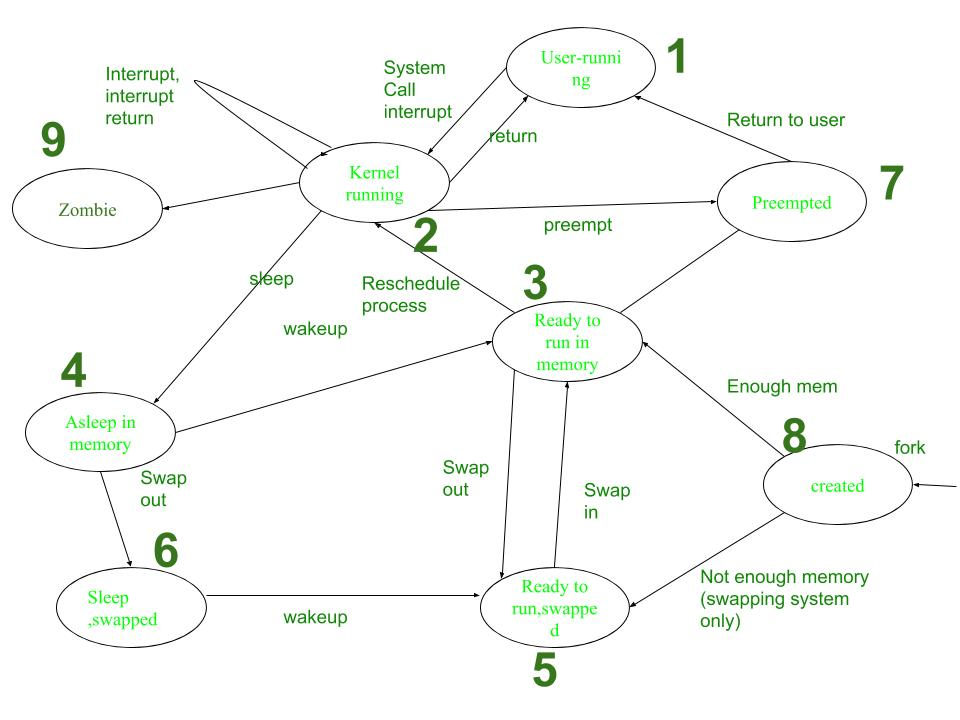
\includegraphics[width=12cm]{images/process/process.jpeg}
    \setcaptioncitation{https://www.geeksforgeeks.org/process-states-and-transitions-in-a-unix-process}
    \caption{Process life cycle in a typical unix system}
    \label{fig:galaxy}
\end{figure}
\end{comment}




\begin{figure}[htp]
    \centering
\tikzset{every picture/.style={line width=0.75pt}} %set default line width to 0.75pt        

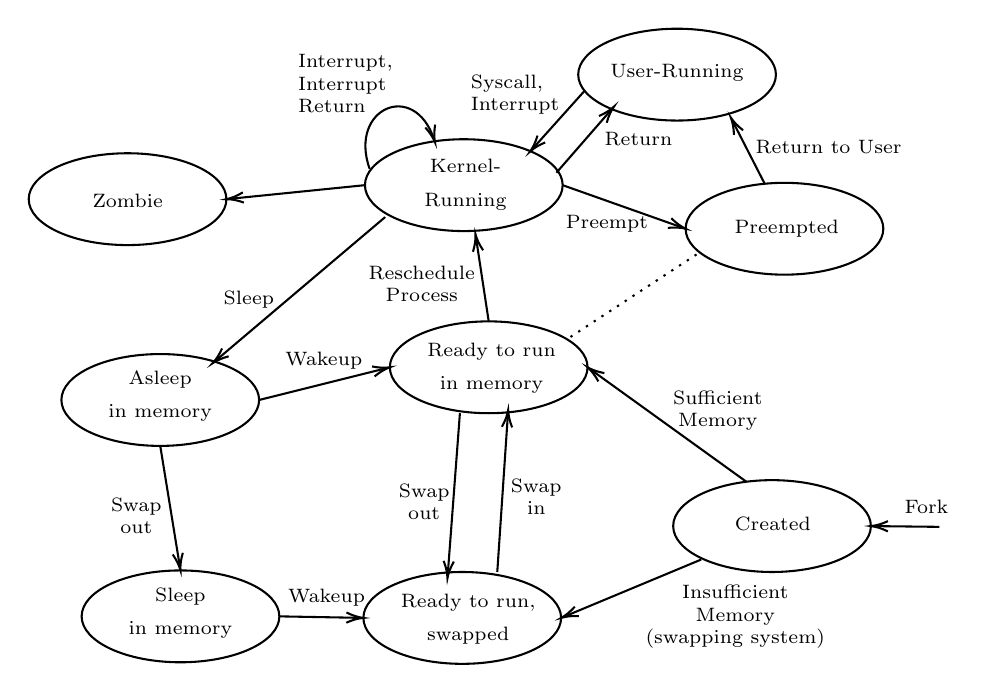
\begin{tikzpicture}[x=0.75pt,y=0.75pt,yscale=-0.75,xscale=0.75]
%uncomment if require: \path (0,505); %set diagram left start at 0, and has height of 505

%Flowchart: Connector [id:dp8160970570643812] 
\draw   (267,248.5) .. controls (267,232.21) and (295.43,219) .. (330.5,219) .. controls (365.57,219) and (394,232.21) .. (394,248.5) .. controls (394,264.79) and (365.57,278) .. (330.5,278) .. controls (295.43,278) and (267,264.79) .. (267,248.5) -- cycle ;
%Flowchart: Connector [id:dp07062083514363515] 
\draw   (457,159.5) .. controls (457,143.21) and (485.43,130) .. (520.5,130) .. controls (555.57,130) and (584,143.21) .. (584,159.5) .. controls (584,175.79) and (555.57,189) .. (520.5,189) .. controls (485.43,189) and (457,175.79) .. (457,159.5) -- cycle ;
%Flowchart: Connector [id:dp18553524714572012] 
\draw   (388,60.5) .. controls (388,44.21) and (416.43,31) .. (451.5,31) .. controls (486.57,31) and (515,44.21) .. (515,60.5) .. controls (515,76.79) and (486.57,90) .. (451.5,90) .. controls (416.43,90) and (388,76.79) .. (388,60.5) -- cycle ;
%Flowchart: Connector [id:dp7880945062151502] 
\draw   (449,350.5) .. controls (449,334.21) and (477.43,321) .. (512.5,321) .. controls (547.57,321) and (576,334.21) .. (576,350.5) .. controls (576,366.79) and (547.57,380) .. (512.5,380) .. controls (477.43,380) and (449,366.79) .. (449,350.5) -- cycle ;
%Flowchart: Connector [id:dp07153592237662654] 
\draw   (250,409.5) .. controls (250,393.21) and (278.43,380) .. (313.5,380) .. controls (348.57,380) and (377,393.21) .. (377,409.5) .. controls (377,425.79) and (348.57,439) .. (313.5,439) .. controls (278.43,439) and (250,425.79) .. (250,409.5) -- cycle ;
%Flowchart: Connector [id:dp8290378636635095] 
\draw   (251,131.5) .. controls (251,115.21) and (279.43,102) .. (314.5,102) .. controls (349.57,102) and (378,115.21) .. (378,131.5) .. controls (378,147.79) and (349.57,161) .. (314.5,161) .. controls (279.43,161) and (251,147.79) .. (251,131.5) -- cycle ;
%Flowchart: Connector [id:dp6001380034764758] 
\draw   (35,140.5) .. controls (35,124.21) and (63.43,111) .. (98.5,111) .. controls (133.57,111) and (162,124.21) .. (162,140.5) .. controls (162,156.79) and (133.57,170) .. (98.5,170) .. controls (63.43,170) and (35,156.79) .. (35,140.5) -- cycle ;
%Flowchart: Connector [id:dp3608424050702036] 
\draw   (56,269.5) .. controls (56,253.21) and (84.43,240) .. (119.5,240) .. controls (154.57,240) and (183,253.21) .. (183,269.5) .. controls (183,285.79) and (154.57,299) .. (119.5,299) .. controls (84.43,299) and (56,285.79) .. (56,269.5) -- cycle ;
%Flowchart: Connector [id:dp1472588739314128] 
\draw   (69,408.5) .. controls (69,392.21) and (97.43,379) .. (132.5,379) .. controls (167.57,379) and (196,392.21) .. (196,408.5) .. controls (196,424.79) and (167.57,438) .. (132.5,438) .. controls (97.43,438) and (69,424.79) .. (69,408.5) -- cycle ;
%Curve Lines [id:da24258380703786953] 
\draw    (254,121) .. controls (240.21,82.12) and (282.69,63.56) .. (295.44,102.2) ;
\draw [shift={(296,104)}, rotate = 253.69] [color={rgb, 255:red, 0; green, 0; blue, 0 }  ][line width=0.75]    (10.93,-3.29) .. controls (6.95,-1.4) and (3.31,-0.3) .. (0,0) .. controls (3.31,0.3) and (6.95,1.4) .. (10.93,3.29)   ;
%Straight Lines [id:da7972175227854316] 
\draw    (251,131.5) -- (163.99,140.3) ;
\draw [shift={(162,140.5)}, rotate = 354.23] [color={rgb, 255:red, 0; green, 0; blue, 0 }  ][line width=0.75]    (10.93,-3.29) .. controls (6.95,-1.4) and (3.31,-0.3) .. (0,0) .. controls (3.31,0.3) and (6.95,1.4) .. (10.93,3.29)   ;
%Straight Lines [id:da14343662453882478] 
\draw    (264,152) -- (154.53,244.71) ;
\draw [shift={(153,246)}, rotate = 319.74] [color={rgb, 255:red, 0; green, 0; blue, 0 }  ][line width=0.75]    (10.93,-3.29) .. controls (6.95,-1.4) and (3.31,-0.3) .. (0,0) .. controls (3.31,0.3) and (6.95,1.4) .. (10.93,3.29)   ;
%Straight Lines [id:da7814144535871211] 
\draw    (119.5,299) -- (132.18,377.03) ;
\draw [shift={(132.5,379)}, rotate = 260.77] [color={rgb, 255:red, 0; green, 0; blue, 0 }  ][line width=0.75]    (10.93,-3.29) .. controls (6.95,-1.4) and (3.31,-0.3) .. (0,0) .. controls (3.31,0.3) and (6.95,1.4) .. (10.93,3.29)   ;
%Straight Lines [id:da22986834689597324] 
\draw    (196,408.5) -- (248,409.46) ;
\draw [shift={(250,409.5)}, rotate = 181.06] [color={rgb, 255:red, 0; green, 0; blue, 0 }  ][line width=0.75]    (10.93,-3.29) .. controls (6.95,-1.4) and (3.31,-0.3) .. (0,0) .. controls (3.31,0.3) and (6.95,1.4) .. (10.93,3.29)   ;
%Straight Lines [id:da5183246324311807] 
\draw    (183,269.5) -- (265.06,248.99) ;
\draw [shift={(267,248.5)}, rotate = 165.96] [color={rgb, 255:red, 0; green, 0; blue, 0 }  ][line width=0.75]    (10.93,-3.29) .. controls (6.95,-1.4) and (3.31,-0.3) .. (0,0) .. controls (3.31,0.3) and (6.95,1.4) .. (10.93,3.29)   ;
%Straight Lines [id:da36938160925280306] 
\draw    (312,278) -- (304.15,382.01) ;
\draw [shift={(304,384)}, rotate = 274.32] [color={rgb, 255:red, 0; green, 0; blue, 0 }  ][line width=0.75]    (10.93,-3.29) .. controls (6.95,-1.4) and (3.31,-0.3) .. (0,0) .. controls (3.31,0.3) and (6.95,1.4) .. (10.93,3.29)   ;
%Straight Lines [id:da1895995011282201] 
\draw    (336,380) -- (342.87,278) ;
\draw [shift={(343,276)}, rotate = 93.85] [color={rgb, 255:red, 0; green, 0; blue, 0 }  ][line width=0.75]    (10.93,-3.29) .. controls (6.95,-1.4) and (3.31,-0.3) .. (0,0) .. controls (3.31,0.3) and (6.95,1.4) .. (10.93,3.29)   ;
%Straight Lines [id:da5028228919093697] 
\draw    (467,372) -- (378.85,408.73) ;
\draw [shift={(377,409.5)}, rotate = 337.38] [color={rgb, 255:red, 0; green, 0; blue, 0 }  ][line width=0.75]    (10.93,-3.29) .. controls (6.95,-1.4) and (3.31,-0.3) .. (0,0) .. controls (3.31,0.3) and (6.95,1.4) .. (10.93,3.29)   ;
%Straight Lines [id:da15122238928340714] 
\draw    (496,322) -- (395.62,249.67) ;
\draw [shift={(394,248.5)}, rotate = 35.78] [color={rgb, 255:red, 0; green, 0; blue, 0 }  ][line width=0.75]    (10.93,-3.29) .. controls (6.95,-1.4) and (3.31,-0.3) .. (0,0) .. controls (3.31,0.3) and (6.95,1.4) .. (10.93,3.29)   ;
%Straight Lines [id:da9119462488777964] 
\draw  [dash pattern={on 0.84pt off 2.51pt}]  (464,176) -- (380,231) ;
%Straight Lines [id:da08612669312273191] 
\draw    (378,131.5) -- (455.11,158.83) ;
\draw [shift={(457,159.5)}, rotate = 199.52] [color={rgb, 255:red, 0; green, 0; blue, 0 }  ][line width=0.75]    (10.93,-3.29) .. controls (6.95,-1.4) and (3.31,-0.3) .. (0,0) .. controls (3.31,0.3) and (6.95,1.4) .. (10.93,3.29)   ;
%Straight Lines [id:da9129325725415524] 
\draw    (508,131) -- (486.91,89.78) ;
\draw [shift={(486,88)}, rotate = 62.9] [color={rgb, 255:red, 0; green, 0; blue, 0 }  ][line width=0.75]    (10.93,-3.29) .. controls (6.95,-1.4) and (3.31,-0.3) .. (0,0) .. controls (3.31,0.3) and (6.95,1.4) .. (10.93,3.29)   ;
%Straight Lines [id:da9605770765837162] 
\draw    (374,123.5) -- (409.69,82.51) ;
\draw [shift={(411,81)}, rotate = 131.04] [color={rgb, 255:red, 0; green, 0; blue, 0 }  ][line width=0.75]    (10.93,-3.29) .. controls (6.95,-1.4) and (3.31,-0.3) .. (0,0) .. controls (3.31,0.3) and (6.95,1.4) .. (10.93,3.29)   ;
%Straight Lines [id:da6816726572039686] 
\draw    (392,71) -- (358.34,108.51) ;
\draw [shift={(357,110)}, rotate = 311.91] [color={rgb, 255:red, 0; green, 0; blue, 0 }  ][line width=0.75]    (10.93,-3.29) .. controls (6.95,-1.4) and (3.31,-0.3) .. (0,0) .. controls (3.31,0.3) and (6.95,1.4) .. (10.93,3.29)   ;
%Straight Lines [id:da11655688316633739] 
\draw    (330.5,219) -- (322.3,164.98) ;
\draw [shift={(322,163)}, rotate = 81.37] [color={rgb, 255:red, 0; green, 0; blue, 0 }  ][line width=0.75]    (10.93,-3.29) .. controls (6.95,-1.4) and (3.31,-0.3) .. (0,0) .. controls (3.31,0.3) and (6.95,1.4) .. (10.93,3.29)   ;
%Straight Lines [id:da026693159156937374] 
\draw    (620,351) -- (578,350.52) ;
\draw [shift={(576,350.5)}, rotate = 0.65] [color={rgb, 255:red, 0; green, 0; blue, 0 }  ][line width=0.75]    (10.93,-3.29) .. controls (6.95,-1.4) and (3.31,-0.3) .. (0,0) .. controls (3.31,0.3) and (6.95,1.4) .. (10.93,3.29)   ;

% Text Node
\draw (277,231) node [anchor=north west][inner sep=0.75pt]  [font=\normalsize] [align=left] {\begin{minipage}[lt]{60pt}\setlength\topsep{0pt}
\begin{center}
{\scriptsize Ready to run \\ \scriptsize in memory}
\end{center}

\end{minipage}};
% Text Node
\draw (485,152) node [anchor=north west][inner sep=0.75pt]   [align=left] {\begin{minipage}[lt]{39.31pt}\setlength\topsep{0pt}
\begin{center}
{\scriptsize Preempted}
\end{center}

\end{minipage}};
% Text Node
\draw (406,52) node [anchor=north west][inner sep=0.75pt]   [align=left] {\begin{minipage}[lt]{48.88pt}\setlength\topsep{0pt}
\begin{center}
{\scriptsize User-Running}
\end{center}

\end{minipage}};
% Text Node
\draw (485,343) node [anchor=north west][inner sep=0.75pt]   [align=left] {\begin{minipage}[lt]{29.34pt}\setlength\topsep{0pt}
\begin{center}
{\scriptsize Created}
\end{center}

\end{minipage}};
% Text Node
\draw (262,392) node [anchor=north west][inner sep=0.75pt]   [align=left] {\begin{minipage}[lt]{60pt}\setlength\topsep{0pt}
\begin{center}
{\scriptsize Ready to run,}\\{\scriptsize swapped}
\end{center}

\end{minipage}};
% Text Node
\draw (265,113) node [anchor=north west][inner sep=0.75pt]   [align=left] {\begin{minipage}[lt]{54.7pt}\setlength\topsep{0pt}
\begin{center}
{\scriptsize Kernel-Running}
\end{center}

\end{minipage}};
% Text Node
\draw (72,135) node [anchor=north west][inner sep=0.75pt]   [align=left] {\begin{minipage}[lt]{27.67pt}\setlength\topsep{0pt}
\begin{center}
{\scriptsize Zombie}
\end{center}

\end{minipage}};
% Text Node
\draw (84,249) node [anchor=north west][inner sep=0.75pt]   [align=left] {\begin{minipage}[lt]{37.63pt}\setlength\topsep{0pt}
\begin{center}
{\scriptsize Asleep}\\{\scriptsize in memory}
\end{center}

\end{minipage}};
% Text Node
\draw (97,388) node [anchor=north west][inner sep=0.75pt]   [align=left] {\begin{minipage}[lt]{37.63pt}\setlength\topsep{0pt}
\begin{center}
{\scriptsize Sleep}\\{\scriptsize in memory}
\end{center}

\end{minipage}};
% Text Node
\draw (206,45.65) node [anchor=north west][inner sep=0.75pt]  [font=\scriptsize] [align=left] {Interrupt,\\Interrupt\\Return};
% Text Node
\draw (317,58.65) node [anchor=north west][inner sep=0.75pt]  [font=\scriptsize] [align=left] {Syscall,\\Interrupt};
% Text Node
\draw (403,95.65) node [anchor=north west][inner sep=0.75pt]  [font=\scriptsize] [align=left] {Return};
% Text Node
\draw (500,100.65) node [anchor=north west][inner sep=0.75pt]  [font=\scriptsize] [align=left] {Return to User};
% Text Node
\draw (378,149) node [anchor=north west][inner sep=0.75pt]  [font=\scriptsize] [align=left] {Preempt};
% Text Node
\draw (248,181.65) node [anchor=north west][inner sep=0.75pt]  [font=\scriptsize] [align=left] {\begin{minipage}[lt]{42.22pt}\setlength\topsep{0pt}
\begin{center}
Reschedule\\Process
\end{center}

\end{minipage}};
% Text Node
\draw (155,197.65) node [anchor=north west][inner sep=0.75pt]  [font=\scriptsize] [align=left] {\begin{minipage}[lt]{21.86pt}\setlength\topsep{0pt}
\begin{center}
Sleep
\end{center}

\end{minipage}};
% Text Node
\draw (196,237) node [anchor=north west][inner sep=0.75pt]  [font=\scriptsize] [align=left] {\begin{minipage}[lt]{29.89pt}\setlength\topsep{0pt}
\begin{center}
Wakeup
\end{center}

\end{minipage}};
% Text Node
\draw (72,330.65) node [anchor=north west][inner sep=0.75pt]  [font=\scriptsize] [align=left] {\begin{minipage}[lt]{33.92pt}\setlength\topsep{0pt}
\begin{center}
Swap\\out
\end{center}

\end{minipage}};
% Text Node
\draw (199,388.65) node [anchor=north west][inner sep=0.75pt]  [font=\scriptsize] [align=left] {\begin{minipage}[lt]{28.51pt}\setlength\topsep{0pt}
\begin{center}
Wakeup
\end{center}

\end{minipage}};
% Text Node
\draw (268,321.65) node [anchor=north west][inner sep=0.75pt]  [font=\scriptsize] [align=left] {\begin{minipage}[lt]{21.44pt}\setlength\topsep{0pt}
\begin{center}
Swap\\out
\end{center}

\end{minipage}};
% Text Node
\draw (340,318.65) node [anchor=north west][inner sep=0.75pt]  [font=\scriptsize] [align=left] {\begin{minipage}[lt]{21.44pt}\setlength\topsep{0pt}
\begin{center}
Swap\\in
\end{center}

\end{minipage}};
% Text Node
\draw (446,261.65) node [anchor=north west][inner sep=0.75pt]  [font=\scriptsize] [align=left] {\begin{minipage}[lt]{33.36pt}\setlength\topsep{0pt}
\begin{center}
Sufficient\\Memory
\end{center}

\end{minipage}};
% Text Node
\draw (427,386.65) node [anchor=north west][inner sep=0.75pt]  [font=\scriptsize] [align=left] {\begin{minipage}[lt]{67.44pt}\setlength\topsep{0pt}
\begin{center}
Insufficient Memory\\(swapping system)
\end{center}

\end{minipage}};
% Text Node
\draw (594,332) node [anchor=north west][inner sep=0.75pt]  [font=\scriptsize] [align=left] {\begin{minipage}[lt]{17.68pt}\setlength\topsep{0pt}
\begin{center}
Fork
\end{center}
\end{minipage}};
\end{tikzpicture}
    \caption[Process life cycle in a typical unix system]{Process life cycle in a typical unix system\footnotemark}
    \label{fig:galaxy}
\end{figure}
\footnotetext{Adapted from \href{https://www.geeksforgeeks.org/process-states-and-transitions-in-a-unix-process}{GeeksforGeeks: Process states and Transitions in a UNIX Process}}

\subsection{Process management}
In our operating system, the management of processes is entrusted to the \texttt{process manager}, a crucial component responsible for overseeing their execution. To facilitate this management, each core within the system maintains a linked list that encompasses comprehensive information about all the processes currently running.

This \href{https://en.wikipedia.org/wiki/Linked_list}{\texttt{linked list}} serves as a repository where data pertaining to various processes, such as their names and statuses, are stored. By traversing this list iteratively, we gain the ability to search for a specific process based on its given name. This search operation allows us to locate the desired process swiftly and efficiently, enabling us to access and modify its status as needed.

To ensure the uniqueness and identification of each process, a unique identifier, known as the \texttt{process ID (PID)}, is assigned to every process. This \texttt{PID} acts as a kind of \texttt{primary key}, distinguishing one process from another and facilitating their individual \texttt{identification} and management within the system.

\subsubsection{Process manager}

The process manager stores various pieces of information to effectively manage processes, including:

\begin{itemize}
    \item \textbf{Spawninfo}: The process manager stores spawninfo, which comprises essential details about the process, such as its initialization parameters, input/output channels, and other relevant configuration data.

    \item \textbf{LMP Channel}: In order to facilitate effective communication between the process and the system, the process manager maintains a dedicated LMP (Lightweight Message Passing) channel. This channel serves as a conduit through which messages can be exchanged between the process and other system components.

    \item \textbf{Process State}: The process manager keeps track of the state of each process. This information provides an indication of whether the process is actively executing, paused, terminated, or in any other state defined within the process lifecycle.

    \item \textbf{Exit Code}: Upon the completion or termination of a process, the process manager captures and stores the exit code. This code signifies the status or outcome of the process's execution and can be used for error handling or diagnostic purposes.

    \item \textbf{Linked List of Waiting Processes}: A function is available for a process to wait for another process to terminate. To do so, each process has a linked list containing all the processes that are awaiting its termination. Additionally, for each process in the waiting list, the process manager stores a callback function. These callbacks serve as notifications or actions that are triggered once the awaited process finishes its execution.
\end{itemize}


\subsubsection{Software pattern used to modify the state of a process}

In our system, we have various operations we can perform on processes, such as resuming a process, terminating a process, or finding the name of a process. Many of these functions follow a similar pattern. Below is an explanation:

To perform these operations, we rely on a data structure called \texttt{spawn info}. This structure contains important information about a process, including its current state. The first step in these functions is to search for the corresponding \texttt{spawn info} in the data structure. Once we find the \texttt{spawn info}, we can make the necessary modifications, such as changing the state of the process or performing other operations based on the specific function we are executing. This allows us to control the behavior of the process as needed.

To locate the relevant \texttt{spawn info}, we utilize a second routine. This routine iterates over a linked list that contains all the spawn info structures. It searches through the list to find the spawn info associated with the process we are working with. This ensures we have the correct information to perform the desired operation.

This pattern of searching for the spawn info and then applying the required modifications is similar to the concept of \href{https://cplusplus.com/reference/iterator/}{\texttt{iterators}} in C++. In C++, an iterator is an object that allows us to traverse through a \href{https://cplusplus.com/reference/stl/}{\texttt{container}} (in C++), such as a linked list, and access its elements one by one. Similarly, in our system, we iterate over the linked list to find the corresponding spawn info and make the necessary changes.


\begin{lstlisting}[caption={Data structures used for the process management},language=C,frame=single,breaklines]
// Linked list containing the processes waiting for a process to exit
struct proc_mgmt_exit_waiting_proc {
    struct event_closure                resume_fn;
    int                                *exit_code;
    struct proc_mgmt_exit_waiting_proc *next;
};

// Linked list containing all processes information
struct proc_mgmt_element {
    struct spawninfo         *si;
    struct proc_mgmt_exit_waiting_proc *waiting_procs;
    struct proc_mgmt_element *next;
};

// Process manager
struct proc_mgmt_state {
    // recursive mutex used for thread safety
    struct thread_mutex mutex;

    // Number of processes handled by this state
    size_t nb_processes_running;
    // list of all the processes handled
    struct proc_mgmt_element *procs;

    // next pid to be attributed
    domainid_t next_pid;
};
\end{lstlisting}

\begin{algorithm}
\caption{Iterate over process}
\begin{algorithmic}[1]

\Procedure{IterateOverProcesses}{\text{domainid\_t } \text{pid}, \text{void *} \text{parameters}}
\State $\text{err} \gets \text{check\_input()}$
\If{$\text{err\_fail}$}
    \Return $\text{INPUT\_ERROR}$
\EndIf

\State $\text{process\_management\_state} \gets \text{get\_process\_management\_state()}$
\State $\text{spawninfo} \gets \text{search\_process\_by\_pid}(\text{pms}, \text{pid})$

\If {$\text{spawninfo} = \text{NULL}$}
    \State \textbf{return} $\text{spawn\_domain\_not\_found}$
\EndIf

\State \text{apply\_specific\_operation\_on\_process()}
\State \textbf{return} $\text{SYS\_ERR\_OK}$
\EndProcedure

\end{algorithmic}
\end{algorithm}

\begin{algorithm}
\caption{Search process by pid}
\begin{algorithmic}[1]

\Procedure{SearchProcessByPID}{$\text{process\_management\_state, pid}$}

\State \Call{Lock()}{}
\State $\text{current\_process\_management\_element} \gets \text{process\_management\_state}\rightarrow \text{proccess\_management\_element}$


\While{$\text{current\_process\_management\_element} \neq \text{NULL}$}
    \If{$\text{current\_process\_management\_element}\rightarrow \text{pid} = \text{pid}$}
        \State \Call{Unlock()}{}
        \State \textbf{return} $\text{current\_process\_management\_element}\rightarrow \text{si}$
    \EndIf
    \State $\text{current\_process\_management\_element} \gets \text{current\_process\_management\_element}\rightarrow \text{next}$
\EndWhile


\State \Call{Unlock()}{}
\EndProcedure

\end{algorithmic}
\end{algorithm}

\subsubsection{Multicore management}

Managing processes on a \texttt{multicore system} is more intricate compared to a single-core system. It requires an efficient approach to gather resources and direct requests to the appropriate destinations. In a multicore setup, each core has its \texttt{own process manager} that is responsible for handling only the processes running on that specific core.

To facilitate this management, \texttt{the process manager} uses the last two digits of the PID (process identifier) to determine which core a process belongs to. In our system, we have up to four cores, so these last two digits of the PID indicate the specific core number. This way, we can easily keep track of which core is responsible for running each process.It's important to note that processes cannot migrate or move between cores.

The process manager on each core focuses solely on the processes running on that particular core. When a request is received, the process manager first checks if it can be fulfilled on the same core. If the request requires resources or actions from another core, \texttt{a remote procedure call} is sent to the corresponding core.

These RPC requests are promptly forwarded when they reach the initialization RPC handler of the incorrect core. This ensures that requests are efficiently \texttt{redirected} to the appropriate core for processing.

In summary, on our \texttt{multicore system}, each core has its \texttt{own process manager}, and processes are confined to their respective cores. Process managers handle requests locally whenever possible, but if resources or actions from another core are needed, RPC calls are sent to the appropriate core to fulfill the request.

\section{Retrospective}
Our process management system has served us very well throughout the process of building our OS. We haven't had any issues with it, and, were we to design it again, we would choose a similar approach.
